\begin{figure*}[t]
  \centering
  % Smiling females missing
%   \normalsize{Missing source: smiling females}\par\medskip
%  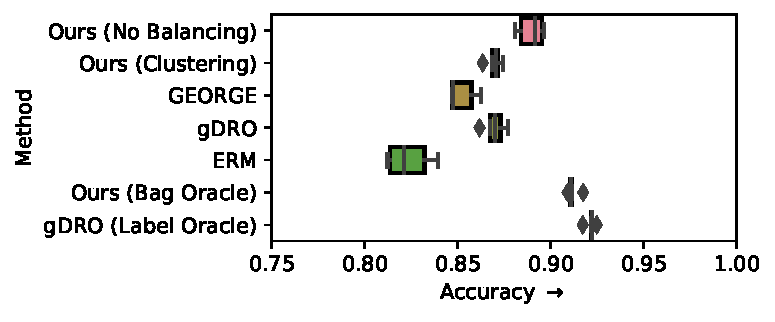
\includegraphics[width=0.49\textwidth, height=3cm]{supmatch/figures/celeba/no_smiling_females/celeba_gender_smiling_acc.pdf}
 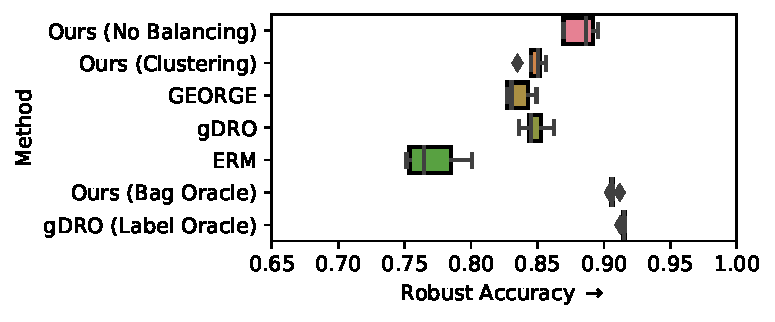
\includegraphics[width=0.49\textwidth]{supmatch/figures/celeba/no_smiling_females/celeba_gender_smiling_acc-min.pdf}
    % Smiling males missing
%   \normalsize{Missing source: smiling males}\par\medskip
%  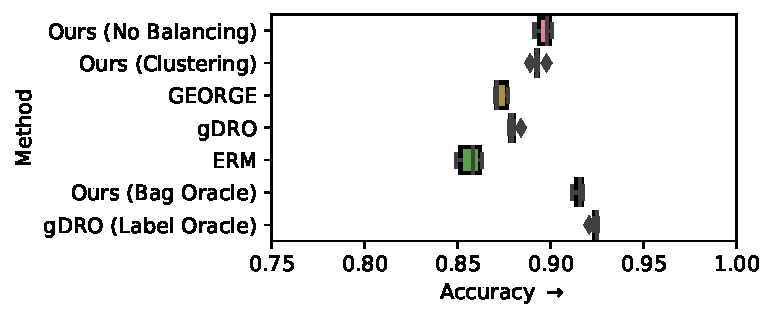
\includegraphics[width=0.49\textwidth]{supmatch/figures/celeba/no_smiling_males/celeba_gender_smiling_acc.pdf}
 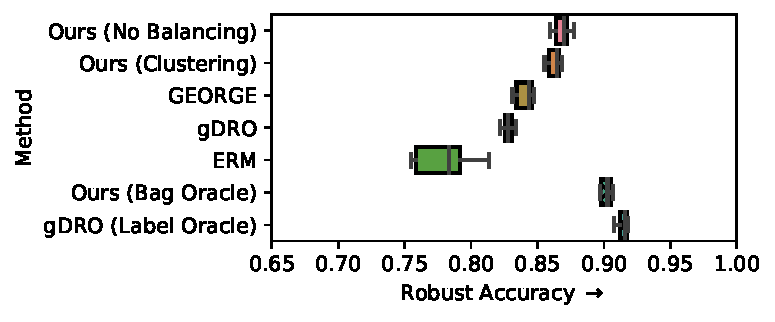
\includegraphics[width=0.49\textwidth]{supmatch/figures/celeba/no_smiling_males/celeba_gender_smiling_acc-min.pdf}
    % Unsmiling females missing
%   \normalsize{Missing source: non-smiling} females\par\medskip
%  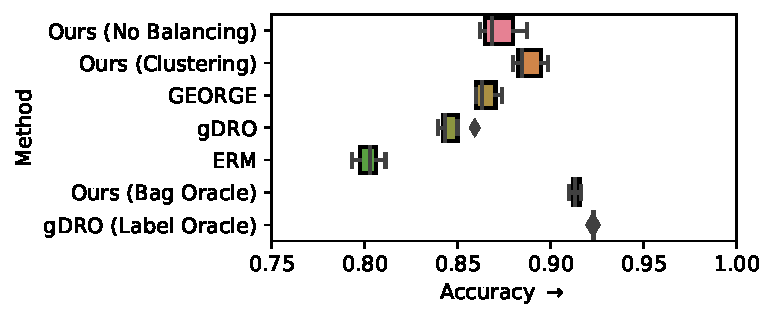
\includegraphics[width=0.49\textwidth]{supmatch/figures/celeba/no_unsmiling_females/celeba_gender_smiling_acc.pdf}
 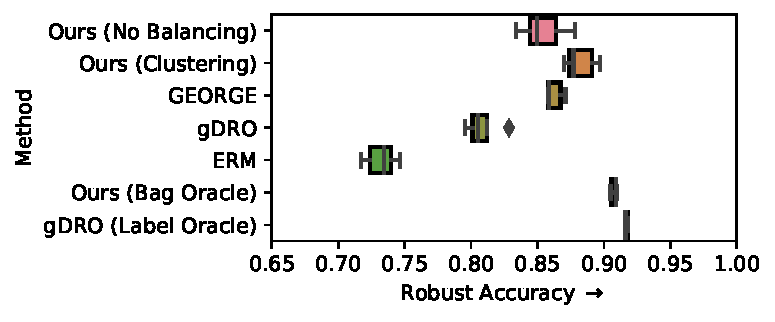
\includegraphics[width=0.49\textwidth]{supmatch/figures/celeba/no_unsmiling_females/celeba_gender_smiling_acc-min.pdf}
  % Unsmiling males missing
%   \normalsize{Missing source: non-smiling males}\par\medskip
%  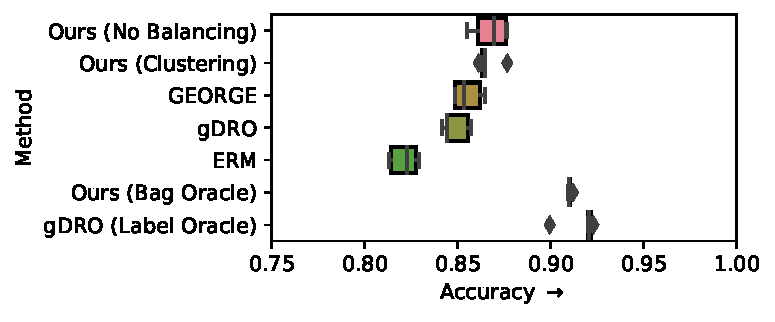
\includegraphics[width=0.49\textwidth]{supmatch/figures/celeba/no_unsmiling_males/celeba_gender_smiling_acc.pdf}
 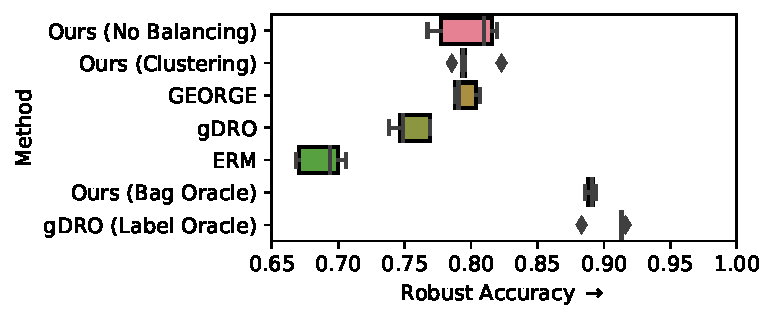
\includegraphics[width=0.49\textwidth]{supmatch/figures/celeba/no_unsmiling_males/celeba_gender_smiling_acc-min.pdf}

% compressed figures:
%   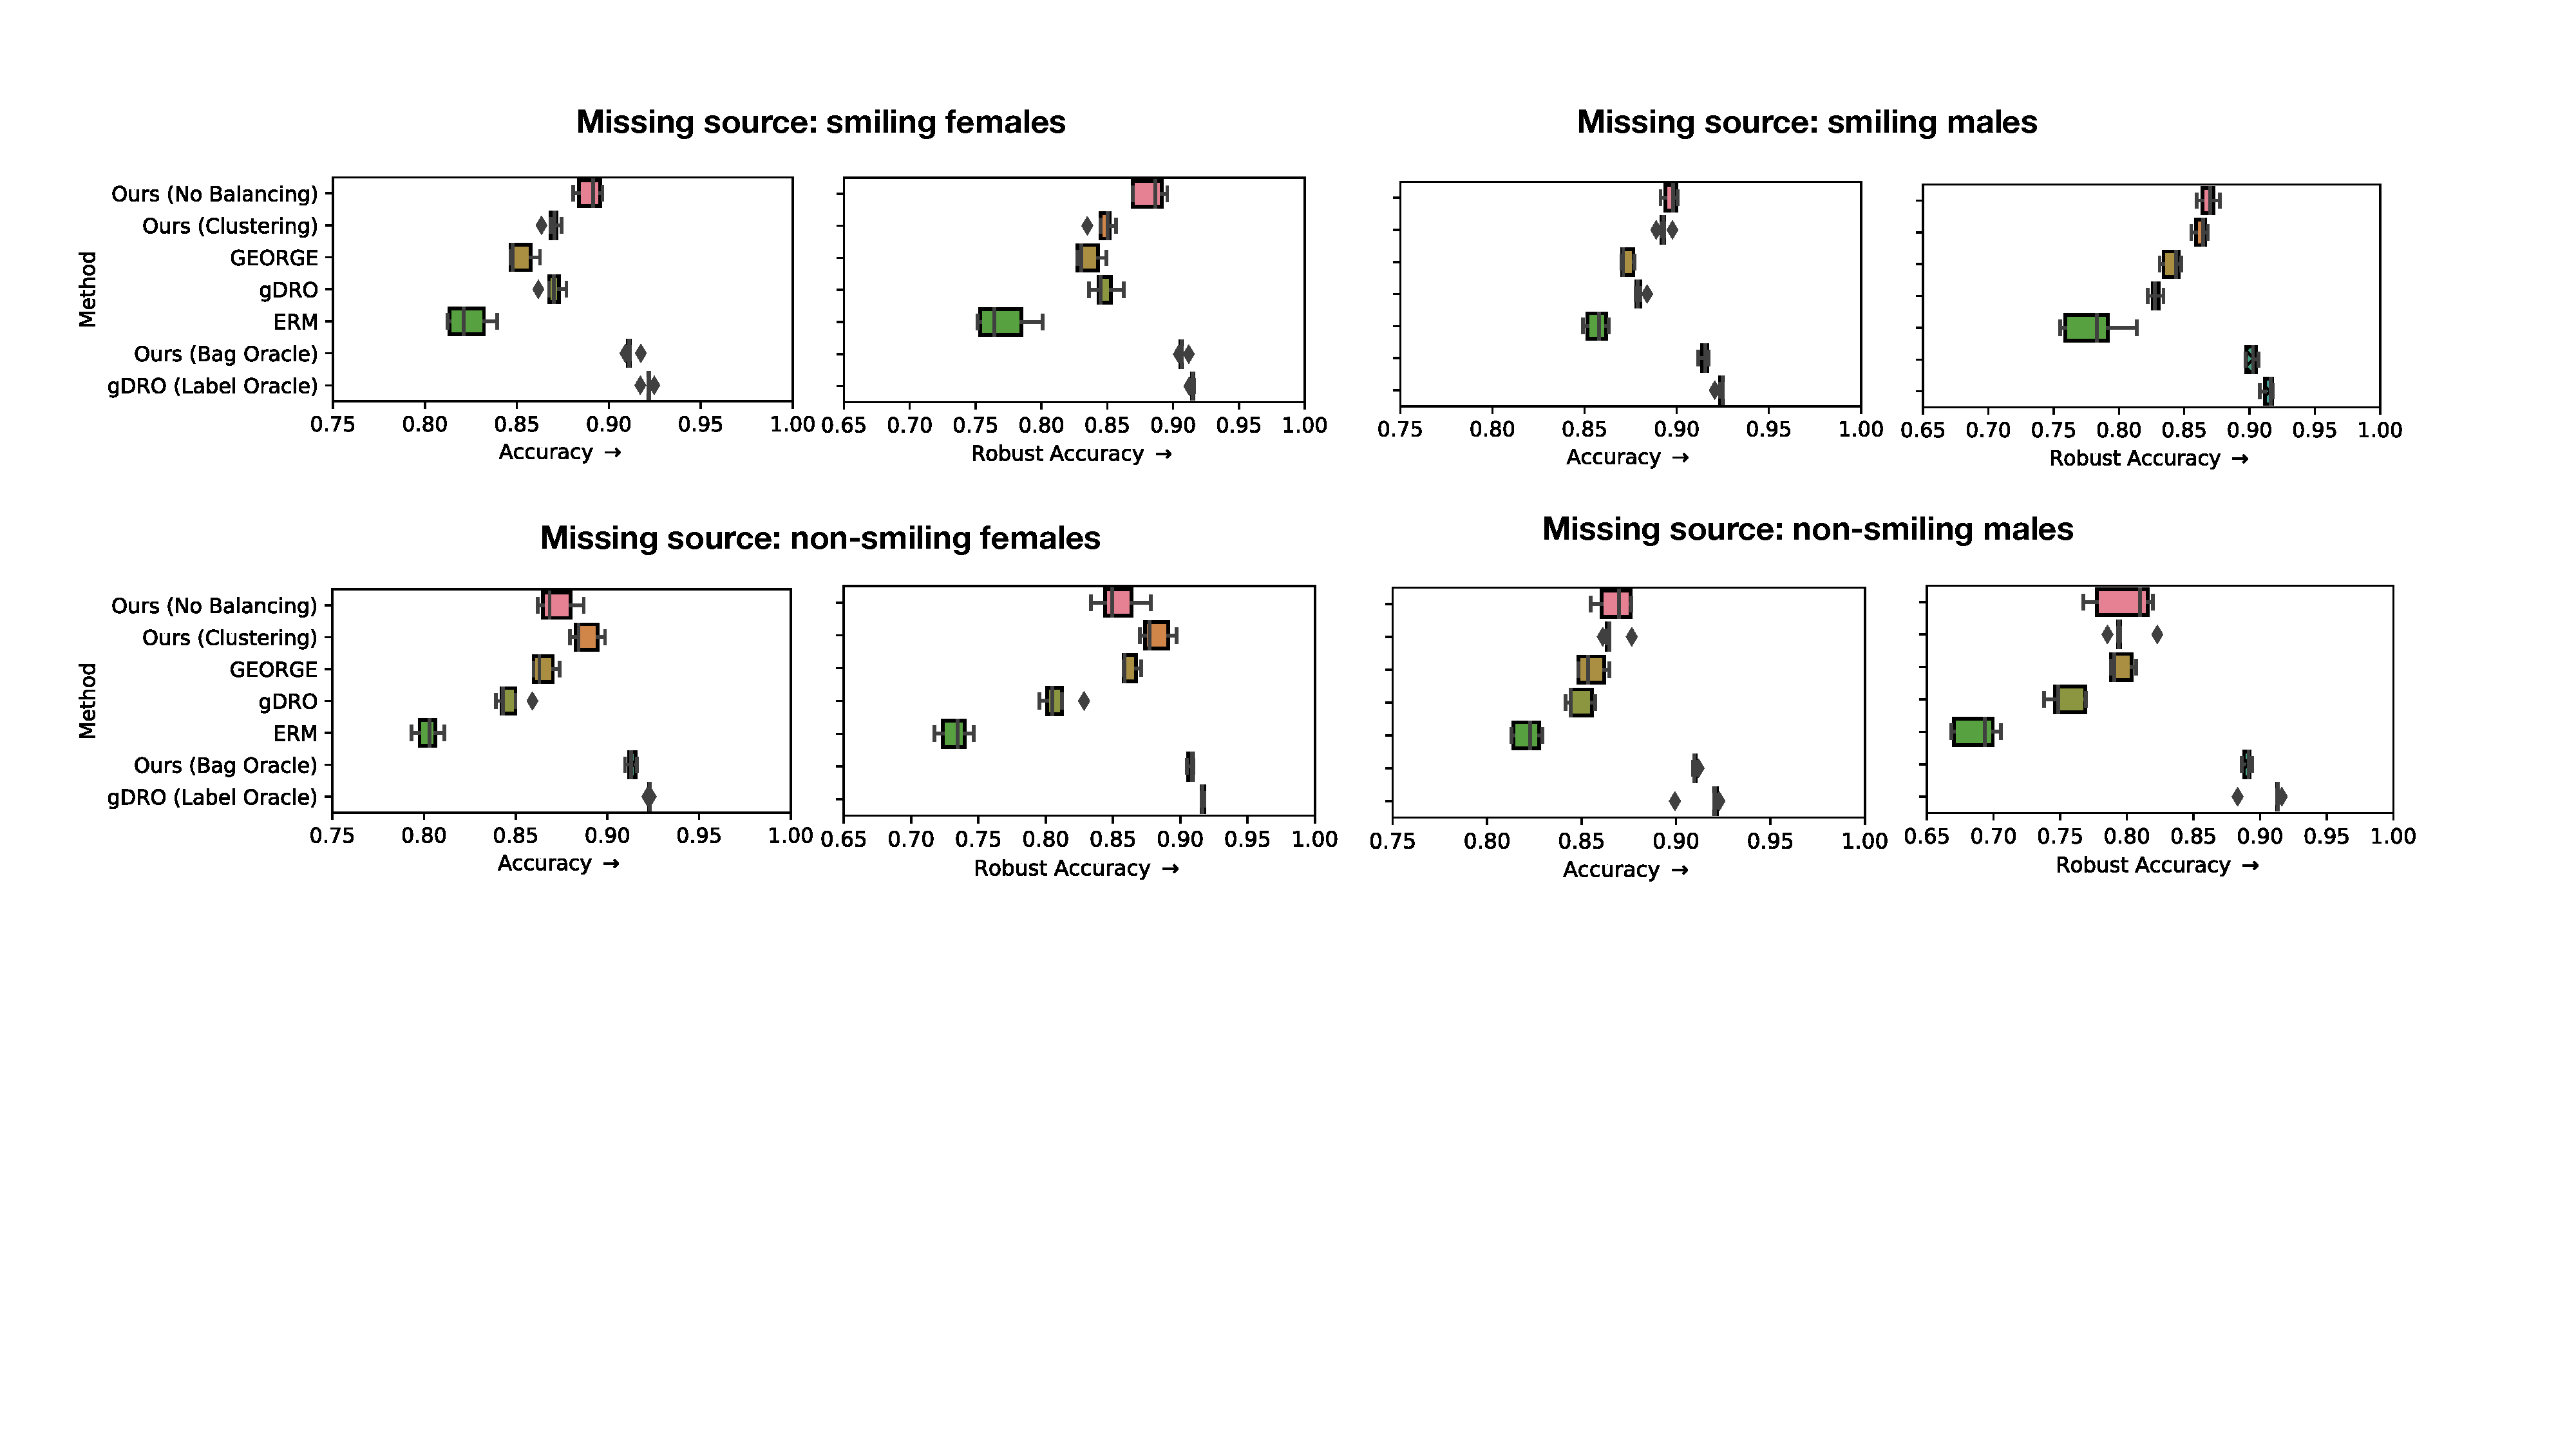
\includegraphics[width=1.0\textwidth]{supmatch/figures/celeba/CelebA2.pdf}
  \caption{
    Results from \textbf{5 repeats} for the CelebA dataset for the \emph{subgroup bias} scenario.
    The task is to predict ``smiling'' vs ``non-smiling'' and the subgroups are based on gender. 
    %
    The four sources are dropped one at a time from the training set
    (\textbf{Top Left}: smiling females; \textbf{Top Right}: smiling males; \textbf{Bottom Left}: non-smiling females;
    \textbf{Bottom Right}: non-smiling males), while the deployment set is kept fixed.
    %
    \texttt{Robust Accuracy} refers to the minimum accuracy computed over the subgroups.
    %
    Our method consistently performs on par with or outperforms \texttt{GEORGE} (which in turn outperforms \texttt{ERM}).
    %
    We note that in some of the runs, \texttt{GEORGE} performed no better than random -- these results were truncated for visibility but can be found in
    Fig.~\ref{fig:celeba-gender-smiling-full}.
    %
    % Due to poor clustering accuracy and the fact that the deployment set is naturally relatively well-balanced with respect to gender, \texttt{Ours (Clustering)} failed to improve on \texttt{Ours (No Balancing)} for all but one missing source.
    %
    Given \emph{indirect} supervision from the deployment set in the form of oracle-balancing, our method performs similarly to \texttt{gDro (Label Oracle)} that receives \emph{direct} supervision.
  }%
  \label{fig:celeba-gender-smiling}
\end{figure*}

